\chapter{Spazio latente}

In machine learning, a latent space, also known as a latent feature space or embedding space, is an abstract space where data is represented in a way that captures underlying patterns and structures1.
The term “latent” refers to the hidden or non-observable features that are inferred from the observable data. 
The concept of latent space is particularly important in unsupervised learning methods such as clustering, dimensionality reduction, and generative models.
Here is an example to illustrate the concept: Imagine we have a large dataset containing names of fruits, animals, cities, and cars.
We realize that storing and training with text data is too expensive, so we decide to map every string to a number.
However, we do not do this randomly. Instead, we map our elements in a way that similar items are closer to each other in the latent space. 
For instance, lemons are closer to oranges than grapes and Lamborghinis. This mapping creates a latent space embedding.


The concept of latent space is crucial in many areas of machine learning and it allows us to capture the essence of data in a lower-dimensional space
and can lead to more efficient computations and improved model performance.

Una tecnica trasversale a diverse applicazioni del \emph{machine learning} (modelli generativi, autoencoders, inferenza variazionale) è l'introduzione 
preliminare di uno spazio latente come artificio atto a ridurre la dimensionalità dello spazio dei dati di ingresso (\emph{input space}).
Lavorare con i dati grezzi, senza un'elaborazione preliminare, risulta computazionalmente oneroso ela capacità di generalizzazione del modello a causa nonché della ridondanza insita negli stessi. 
Lavorre con i dati grezzi infica la capacità di generalizzazione del modello nonché il tempo di apprendimento.

Lo spazio latente può essere visto come una reppresntazione compressa dei dati, nel quale dati simili sono 
 These features or variables \emph{variabili latenti} are called "latent variables" dal momento che non sono direttamente osservabili nei dati, ma vengono dedotte da quest'ultimi. 

  Latent spaces are used in a variety of machine learning tasks, such as dimensionality reduction, generative models, and clustering. 
  They can be used to identify pattern o strutture ricorrenti nei dati che patterns or structure in the data that would be difficult to detect using other methods. 
For example, a latent space might be used to represent the underlying structure of an image dataset, such as the position and shape of objects in the images.


Si supponga di disporre di un dataset composto da immagini in scala di grigi di scatole di oggetti (\ref{fig:t7ui}).
A un osservatore umano per ispezione due carateristiche (\emph{features}) che possono rappresentare univocamente ogni elemento del suddetto
dataset: l'\emph{altezza} e la \emph{larghezza} della scatola. Pertanto è possibile 



transformation of data from a high-dimensional space into a low-dimensional space so that the low-dimensional 
representation retains some meaningful properties of the original data, ideally close to its intrinsic dimension.

A latent space refers to a conceptual space or representation in which data points are encoded as a set of latent variables or hidden factors. 
These latent variables are not directly observable in the data but are inferred or learned from it. 
The latent space is often of lower dimensionality than the original feature space and aims to capture the underlying structure or patterns in the data in a more compact and meaningful form.
In l'obiettivo è quello di apprendere un'applicazione, nell'accezione matematica del termine, dallo spazio del dati ad un opportuno spazio latente

In various machine learning techniques, such as generative models, autoencoders, or variational inference, the goal is to learn a mapping from the original data space to a latent space. 
This mapping allows for efficient representation and manipulation of the data by reducing its dimensionality and capturing the most relevant information.
The term "latent" implies that these variables are hidden or unobserved, and their values are derived from the observed data through a learning process.
The latent space can be seen as a compressed representation of the data, where similar data points are mapped closer together, enabling tasks like clustering, anomaly detection, data generation,
or interpolation between data points

\begin{figure}
  \centering
  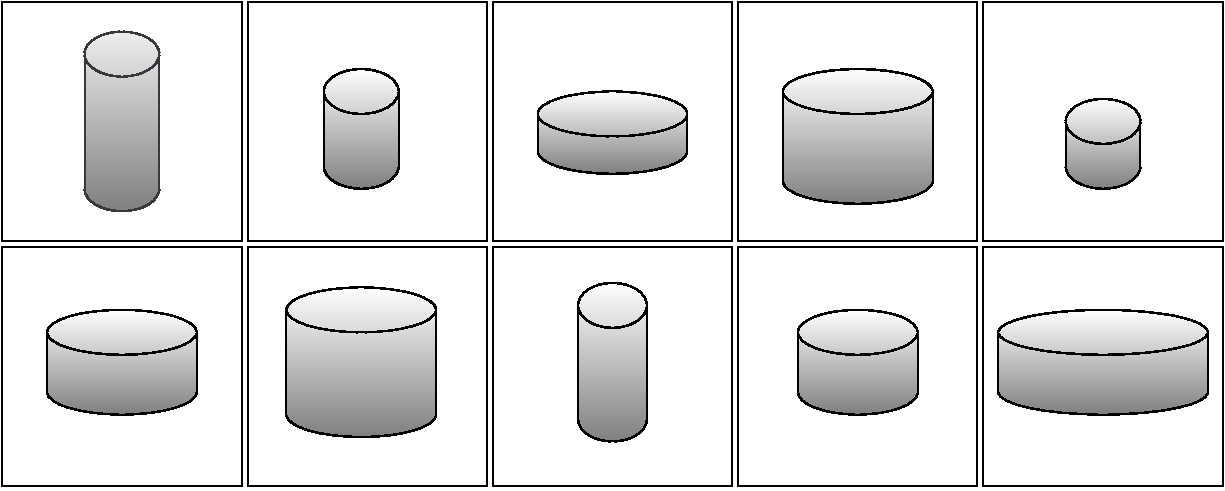
\includegraphics[keepaspectratio, scale=0.45]{Latent_Space1}
  \caption{gviryfkduls, tratto da \cite{davidfosterGenerativeDeepLearning2023}}
  \label{fig:t7ui}
\end{figure}




\begin{figure}
  \centering
  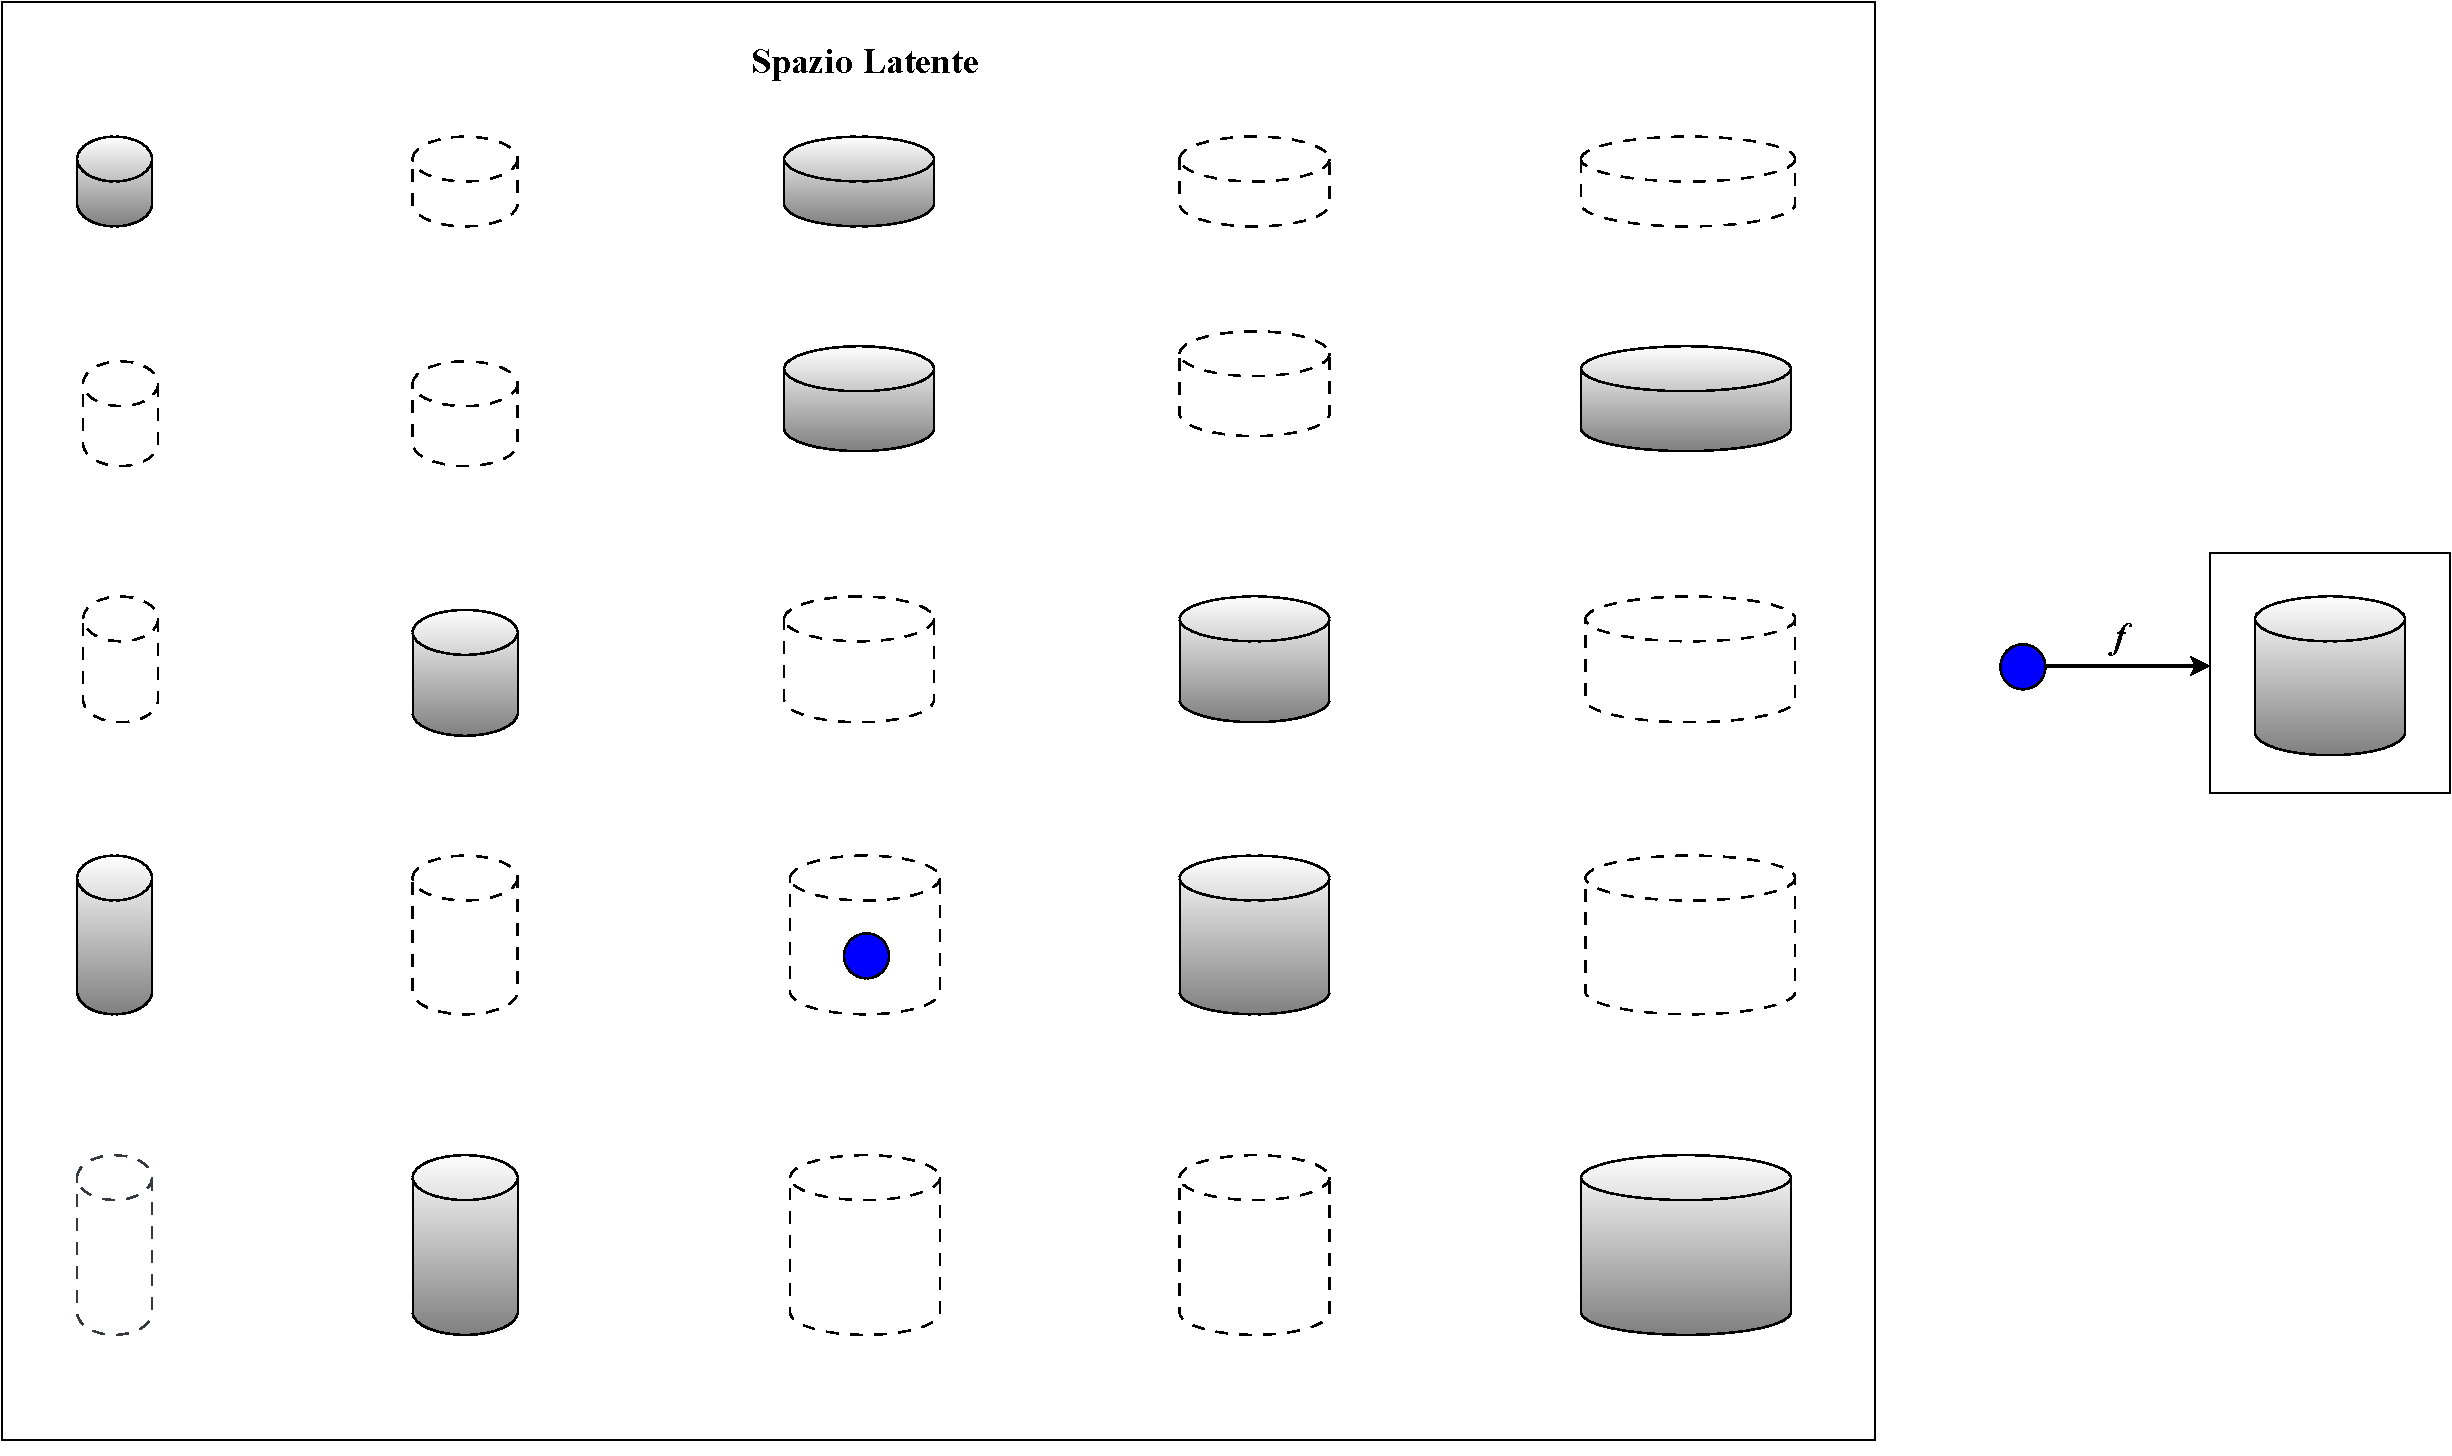
\includegraphics[keepaspectratio, scale=0.3]{Latent_Space2}
  \caption{gviryfkduls, tratto da \cite{davidfosterGenerativeDeepLearning2023}}
\end{figure}